\documentclass[12pt]{article}

\usepackage{se-alexandre}

\usepackage{graphicx,url}

\usepackage[brazil]{babel}   
\usepackage[utf8]{inputenc}  

     
\sloppy

\title{Trabalho da disciplina de Sistemas Evolutivos:\\ A Cellular Automata
 Model of Population Infected by Periodic Plague}

\author{Alexandre G. da Costa\inst{1}}


\address{Centro de Desenvolvimento Tecnológico -- Universidade Federal de
 Pelotas
  (UFPEL)\\
  Pelotas -- RS -- Brasil
  \email{alexandre.costa@inf.ufpel.edu.br}
}

\begin{document} 

% ----------------------------------------------------------------------------
\maketitle

% ----------------------------------------------------------------------------
\begin{abstract}
  This meta-paper describes the style to be used in articles and short papers
  for SBC conferences. For papers in English, you should add just an abstract
  while for the papers in Portuguese, we also ask for an abstract in
  Portuguese (``resumo''). In both cases, abstracts should not have more than
  10 lines and must be in the first page of the paper.
\end{abstract}
  
% ----------------------------------------------------------------------------   
\begin{resumo} 
  Este trabalho descreve a implementação do artigo proposto na disciplina de
  Sistemas Evolutivos e propõe uma nova abordagem da implementação. Esse
  artigo descreve um algoritmo que evolui.
\end{resumo}

% ----------------------------------------------------------------------------
\section{Introdução}

Automato celular é um modelo matemático que foi desenvolvido para simular a
evolução natural, por exemplo \textit{Game of Life}. Pois ele define tanto o
meio ambiante como também os indivíduos.


% ----------------------------------------------------------------------------
\section{Trabalhos Relacionados}
% Nesta sessão será explicado em detalhes o artigo referencial.

O artigo referencial abordado neste trabalho foi \textit{A Cellular Automata 
Model of Population Infected by Periodic Plague} de Witold Dzwinel. Nesse
artigo Dzwinel propõe um modelo complementar ao \textit{Penna paradigm}
\cite{almeida1998theoretical, de1998strategies} que considera a mutação
genética. Esse modelo complementar objetiva analisa a influência de fatores
ambientais sobre o processo de envelhecimento.

O modelo implementado no trabalho de \cite{dzwinel:04} assume que o conjunto
$S(t)$ de indivíduos é jogado aleatória mente em uma matriz, bi-dimensional,
de um Automato Celular (AC). Cada indivíduo fica em uma célula e carrega um
código genético binário Figura \ref{fig:codigo-genetico}.

\begin{figure}[ht]
\centering
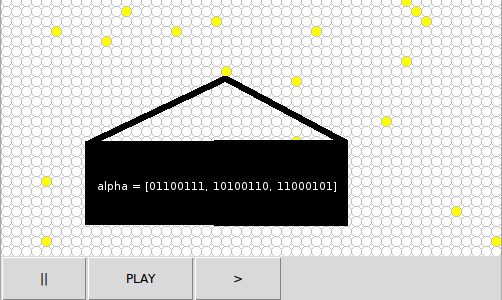
\includegraphics[width=.5\textwidth]{imagens/codigo-genetico}
\caption{Exemplo do código genético de um indivíduo.}
\label{fig:codigo-genetico}
\end{figure}

% ----------------------------------------------------------------------------
\section{Proposta}

Nesta sessão tem o objetivo de explicar o trabalho proposto, ressaltando as
contribuições da proposta.


% ----------------------------------------------------------------------------
\section{Resultados Alcançados}

Se possível comparando com o trabalho referencial.

% ----------------------------------------------------------------------------
\section{Conclusões}

Apresentar as conclusões  \cite{dzwinel:04}.

%\begin{figure}[ht]
%\centering
%\includegraphics[width=.5\textwidth]{fig1.jpg}
%\caption{A typical figure}
%\label{fig:exampleFig1}
%\end{figure}

%\begin{figure}[ht]
%\centering
%\includegraphics[width=.3\textwidth]{fig2.jpg}
%\caption{This figure is an example of a figure caption taking more than one
%  line and justified considering margins mentioned in
% Section~\ref{sec:figs}.}
%\label{fig:exampleFig2}
%\end{figure}

%\begin{table}[ht]
%\centering
%\caption{Variables to be considered on the evaluation of interaction
%  techniques}
%\label{tab:exTable1}
%\includegraphics[width=.7\textwidth]{table.jpg}
%\end{table}

% ----------------------------------------------------------------------------

\bibliographystyle{sbc}
\bibliography{se-alexandre}

\end{document}
